
	\chapter{Delete variable -dv}
	
	If there is variable having only one value, then such a variable can be removed from the problem because it becomes redundant. It is redundant since init sets the variable to its only value and the variable cannot be changed to any other value. Note that the variable can appear only in prevail preconditions. 
	
	\begin{figure}
		\begin{subfigure}[b]{0.4\textwidth}
			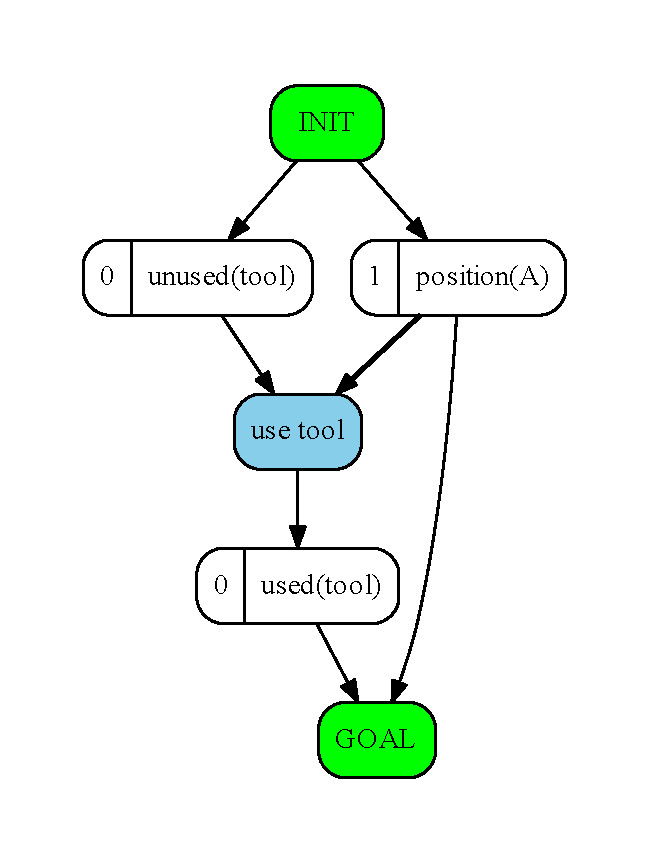
\includegraphics[scale=0.4]{deleteVariable/figures/simple_input}
			\caption{before reduction}
		\end{subfigure}	
		\begin{subfigure}[b]{0.4\textwidth}
			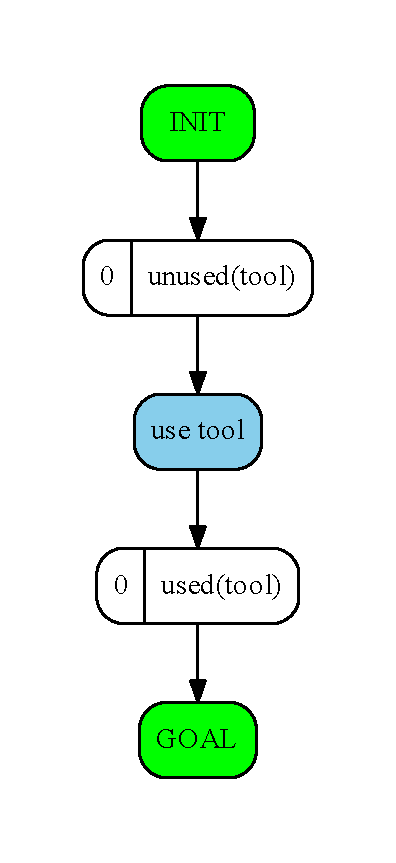
\includegraphics[scale=0.4]{deleteVariable/figures/simple_output}
			\caption{after reduction}
		\end{subfigure}
		\caption{variable 1 can be removed because it becomes redundant as can be seen}
	\end{figure}
	
	
	\section{Reduce operation}
	Let have SAS in form $<\vars, \init, \goal, \actions, \mutexes{}>$. This reduction is performed if there is $v \in \vars: |\dom{v}| = 1$. Let work with such variable $v$.
	
	Let $u$ be the only remaining value of variable $v$. The reduction operation performs following steps: removing $v$ from variables \ref{RV:out:remove}, removing preconditions with $v$ \ref{RV:out:act} (we assume that there are no effects of type $<e,e>$ where $e \in \dom{v}$), removing the value from init \ref{RV:out:init}, goal \ref{RV:out:goal} and mutexes \ref{RV:out:mutex}.
	
	\begin{enumerate}
		\item $\vars{}' \leftarrow \vars \setminus \{v\}$ \label{RV:out:remove}
		\item $\init{}' \leftarrow \init \setminus \{u\}$ \label{RV:out:init}
		\item $\goal{}' \leftarrow \goal \setminus \{u\}$ \label{RV:out:goal}
		\item \begin{enumerate}
			\item $\actions{}_c \leftarrow \{a | a \in \actions, u \in \pre{a}\}$
			\item remove preconditions containing value $u$ from $\actions{}_c$ and store these actions to $\actions{}_d$
			\item $\actions{}' \leftarrow (\actions \setminus \actions{}_c) \cup \actions{}_d$ \label{RV:out:act}
		\end{enumerate}
		\item remove value $u$ from all mutexes and store that with unchanged mutexes to $\mutexes{}'$ \label{RV:out:mutex}
	\end{enumerate}
	
	Output of the reduction is SAS $<\vars{}', \init{}', \goal{}', \actions{}', \mutexes{}'>$.
	
	\section{Possible outgoing states of SAS}
	Following states of SAS can occur after the reduction:
	
	\begin{enumerate}
		\item mutex may be empty after this operation 
		\item state where -mv can be applied may be made
		\item some actions may have fewer preconditions, therefore some actions may be merged together as similar
		\item state where simple dependency may be applied may be made
	\end{enumerate}
	
	\section{States before application of this action}
	\begin{itemize}
		\item -mv can caused this
		\item removing some value, therefore after application of dead ends, one effect reduction or using pruning by -uv
	\end{itemize}
	
	
	\section{Reverse operation}
	The reverse operation is quite simple. The things that were removed during reduction, are added back to the SAS (at all places - in mutexes, operations, init, goal and variables).
	
	
	\section{Implementation notes}
	This operation needs to be run as last one to ensure that FD will not crash.
	
	
	
	
	